% !TeX program = pdflatex
% Original architecture-engineering guidance; no licensed source text embedded.
\documentclass[11pt,letterpaper]{article}
\usepackage[T1]{fontenc}
\usepackage{lmodern,microtype}
\usepackage[margin=0.85in,headheight=16pt]{geometry}
\usepackage[table]{xcolor}
\usepackage{booktabs,tabularx,longtable,array,ragged2e}
\usepackage{tikz}
\usetikzlibrary{positioning,arrows.meta}
\usepackage{enumitem,needspace,fancyhdr,hyperref}
\definecolor{navy}{HTML}{17364D}
\definecolor{teal}{HTML}{087D83}
\definecolor{muted}{HTML}{516371}
\hypersetup{colorlinks=true,linkcolor=teal,urlcolor=teal}
\setlength{\parindent}{0pt}
\setlength{\parskip}{5pt}
\setlength{\emergencystretch}{3em}
\raggedbottom
\setlist{leftmargin=1.5em,itemsep=2pt,topsep=3pt}
\renewcommand{\arraystretch}{1.2}
\newcolumntype{Y}{>{\RaggedRight\arraybackslash}X}
\pagestyle{fancy}\fancyhf{}
\fancyhead[L]{\small\sffamily\color{navy} ARCHITECTURE ENGINEERING}
\fancyhead[R]{\small\sffamily\color{muted} SUITE / 1.0}
\fancyfoot[L]{\small\sffamily\color{muted} V\&B / ISO 42010:2022}
\fancyfoot[R]{\small\thepage}
\newcommand{\docsection}[1]{\Needspace{5\baselineskip}\section{#1}}
\newcommand{\docsub}[1]{\Needspace{4\baselineskip}\subsection{#1}}
\newcommand{\field}[1]{\par\textbf{#1}\par\noindent\rule{\linewidth}{0.3pt}\par\vspace{0.5em}}
\begin{document}
\begin{titlepage}\thispagestyle{empty}\raggedright
\vspace*{0.65in}
{\sffamily\bfseries\color{teal} ARCHITECTURE DOCUMENTATION / WORKED EXAMPLE\par}
\vspace{0.35in}
{\sffamily\bfseries\color{navy}\Huge Reference Software Architecture Document\par}
\vspace{0.2in}
{\sffamily\Large\color{muted} Worked example: repository security-analysis service\par}
\vspace{0.35in}\noindent{\color{teal}\rule{\linewidth}{1.5pt}}\par
\vspace{0.3in}
A fully bounded illustrative design showing stakeholder traceability, module and runtime structures, allocation, behavior, trust boundaries, decisions and cross-view checks. No deployed system or measured results are represented.

\vfill
{\sffamily\small Edition 1.0 \quad / \quad 25 November 2026\par
Status: library working edition \quad / \quad Original engineering guidance\par}
\end{titlepage}
\tableofcontents\clearpage
\docsection{Identity, scope and environment}
AD-REF v1.0 describes a proposed repository security-analysis service. EoI: the service from authenticated job submission to read-only analysis and publication of redacted findings. External entities: developer, identity provider, source repository, ticketing API and infrastructure operator. Excluded: scanner internals, repository write operations, production infrastructure and actual security certification. Purpose: show how a small system can be documented using the suite. All specifications, scenarios and evidence in this example are synthetic; no software was deployed.

Baseline: design revision REF-1. Owner: illustrative architecture team. Status: example. No prior architecture evaluations exist in this fictional project. Resource limit: no implementation, performance test, infrastructure proof or independent stakeholder validation. No positive formal conformance claim. The roadmap follows stakeholder registers, module, runtime, allocation, security/behavior, correspondences and decisions.

\docsection{Stakeholders, perspectives, concerns and aspects}
\begin{longtable}{@{}>{\RaggedRight\arraybackslash}p{0.297\linewidth}>{\RaggedRight\arraybackslash}p{0.297\linewidth}>{\RaggedRight\arraybackslash}p{0.297\linewidth}@{}}
\toprule
\textbf{Stakeholder} & \textbf{Perspective} & \textbf{Concerns}\\\midrule
\endhead
STK-01 Developer & PER-01 Engineering & CON-01 modifiability; CON-02 actionable results\\
STK-02 Operator & PER-02 Operations & CON-03 recovery; CON-04 capacity\\
STK-03 Security reviewer & PER-03 Security & CON-05 authorization; CON-06 auditability\\
\bottomrule
\end{longtable}
\begin{longtable}{@{}>{\RaggedRight\arraybackslash}p{0.297\linewidth}>{\RaggedRight\arraybackslash}p{0.297\linewidth}>{\RaggedRight\arraybackslash}p{0.297\linewidth}@{}}
\toprule
\textbf{Concern} & \textbf{Question and aspect} & \textbf{Viewpoint / view}\\\midrule
\endhead
CON-01 & Can providers be changed independently? ASP-01 structural. & VP-MD, VP-MU / V-01, V-02\\
CON-02 & How does a result reach the developer? ASP-02 behavioral. & VP-CC / V-03\\
CON-03 & How is an accepted job recovered? ASP-02 behavioral. & VP-CC, VP-BH / V-03, V-05\\
CON-04 & Where can workers scale? ASP-03 physical. & VP-DEP / V-04\\
CON-05 & How are tenant boundaries enforced? ASP-04 security. & VP-SEC / V-06\\
CON-06 & How is publication audited? ASP-04 security. & VP-SEC / V-06\\
\bottomrule
\end{longtable}
PER-01 maps to VP-MD, VP-MU and VP-CC; PER-02 to VP-CC, VP-DEP and VP-BH; PER-03 to VP-SEC. All six viewpoints and governing model kinds use version 1.0 of the companion catalog, with actual concerns above replacing typical examples. Viewpoint specifications are referenced as part of this example package, not asserted independently conforming. Selected viewpoints answer structure, execution, placement, failure behavior and trust questions; other styles are omitted because they do not add distinct information for this scope.

\docsection{V-01 / module decomposition}
Version 1.0; VP-MD, VC-01 v1.0 / MK-TREE. Primary presentation: parent M-00 contains M-01 API, M-02 orchestration, M-03 scanner adapter, M-04 persistence adapter, M-05 publisher adapter. Legend L-01: contains denotes implementation ownership, not runtime communication.

\begin{longtable}{@{}>{\RaggedRight\arraybackslash}p{0.297\linewidth}>{\RaggedRight\arraybackslash}p{0.297\linewidth}>{\RaggedRight\arraybackslash}p{0.297\linewidth}@{}}
\toprule
\textbf{Module} & \textbf{Responsibility} & \textbf{Interface}\\\midrule
\endhead
M-01 API & Authenticate and validate requests & I-01 submit/status\\
M-02 Orchestration & Job policy, state transitions and retry decisions & I-02 execute\\
M-03 Scanner adapter & Read source and produce normalized findings & I-03 scan\\
M-04 Persistence adapter & Durable job and finding state & I-04 store\\
M-05 Publisher adapter & Redact and deliver approved findings & I-05 publish\\
\bottomrule
\end{longtable}
Context: repository and ticketing clients are outside core policy. Variability: adapters may change if contracts remain compatible. Rationale ADR-01; known issue ISSUE-01: no source tree or dependency extraction available for proposed structure.

\docsection{V-02 / module uses}
Version 1.0; VP-MU, VC-02 v1.0 / MK-GRAPH. The core orchestration module depends on abstractions within M-02; adapters implement the abstractions. The composition root in M-01 wires concrete adapters. Directed uses relations are represented in the following catalog; implementation imports remain unverified.

\begin{longtable}{@{}>{\RaggedRight\arraybackslash}p{0.297\linewidth}>{\RaggedRight\arraybackslash}p{0.297\linewidth}>{\RaggedRight\arraybackslash}p{0.297\linewidth}@{}}
\toprule
\textbf{Source} & \textbf{Uses target} & \textbf{Reason}\\\midrule
\endhead
M-01 & M-02 & Job API\\
M-01 & M-03, M-04, M-05 & Composition only\\
M-03 & M-02 & Scan port contract\\
M-04 & M-02 & Persistence port contract\\
M-05 & M-02 & Publication port contract\\
\bottomrule
\end{longtable}
M-02 has no concrete-adapter dependency in this design; no directed cycles appear in the declared graph. Rationale ADR-01; context and variability are as V-01. Known issue ISSUE-01: only design evidence, not code.

\docsection{V-03 / runtime interaction}
Version 1.0; VP-CC, VC-03 v1.0 / MK-CC. The primary presentation uses directed arrows for request or work flow only. C-01 API accepts jobs, C-02 worker consumes queued work, C-03 queue, C-04 store and C-05 publisher complete the service. The queue is durable and externally managed; C-04 is managed persistence.

\begin{center}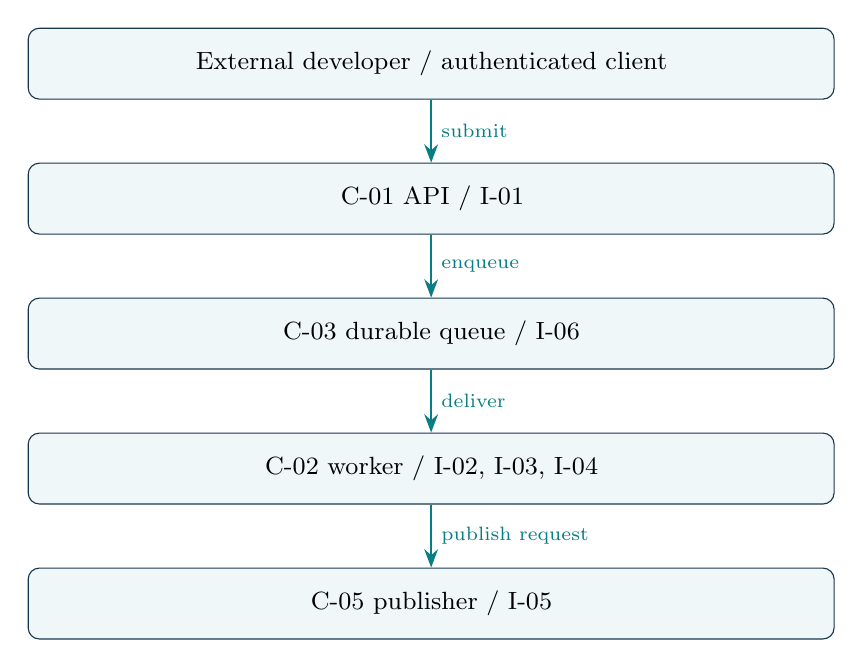
\begin{tikzpicture}[n/.style={draw=navy,rounded corners,fill=teal!6,text width=10cm,align=center,minimum height=9mm,font=\small},>=Stealth]
\node[n] (n0) {External developer / authenticated client};
\node[n,below=8mm of n0] (n1) {C-01 API / I-01};
\node[n,below=8mm of n1] (n2) {C-03 durable queue / I-06};
\node[n,below=8mm of n2] (n3) {C-02 worker / I-02, I-03, I-04};
\node[n,below=8mm of n3] (n4) {C-05 publisher / I-05};
\draw[->,teal,thick] (n0) -- node[right,font=\scriptsize] {submit} (n1);
\draw[->,teal,thick] (n1) -- node[right,font=\scriptsize] {enqueue} (n2);
\draw[->,teal,thick] (n2) -- node[right,font=\scriptsize] {deliver} (n3);
\draw[->,teal,thick] (n3) -- node[right,font=\scriptsize] {publish request} (n4);\end{tikzpicture}\end{center}
\begin{longtable}{@{}>{\RaggedRight\arraybackslash}p{0.457\linewidth}>{\RaggedRight\arraybackslash}p{0.457\linewidth}@{}}
\toprule
\textbf{Connector} & \textbf{Contract and behavior}\\\midrule
\endhead
I-01 client to C-01 & HTTPS; tenant-scoped token; return job ID after durable acceptance.\\
I-06 C-01 to C-03 to C-02 & At-least-once delivery; immutable job ID; duplicate-safe processing.\\
I-03 C-02 to repository & Read-only scoped credential; timeout and retry bounded.\\
I-04 C-01/C-02/C-05 to C-04 & Transactional state and idempotency key; no secret values stored.\\
I-05 C-05 to ticket API & Redacted result, tenant and idempotency key; retry on transient error.\\
\bottomrule
\end{longtable}
Diagram suppresses C-04 and external repository/ticket API for readability; the connector catalog makes their interactions explicit. Worker replicas are interchangeable. Context: untrusted source content is treated as data. Rationale ADR-02 and ADR-03. Known issue ISSUE-02: failure behavior not tested.

\docsection{V-04 / deployment allocation}
Version 1.0; VP-DEP, VC-04 v1.0 / MK-MAP. Allocation targets N-01 application execution zone, N-02 managed queue, N-03 managed database, N-04 publisher execution zone. The design uses private network access and managed encrypted services; no specific provider or capacity is assumed.

\begin{longtable}{@{}>{\RaggedRight\arraybackslash}p{0.297\linewidth}>{\RaggedRight\arraybackslash}p{0.297\linewidth}>{\RaggedRight\arraybackslash}p{0.297\linewidth}@{}}
\toprule
\textbf{Runtime unit} & \textbf{Target} & \textbf{Multiplicity / notes}\\\midrule
\endhead
C-01 API & N-01 & At least two replicas proposed\\
C-02 worker & N-01 & Independent horizontal scaling; bounded concurrency\\
C-03 queue & N-02 & Managed service; retention configured\\
C-04 store & N-03 & Managed database; backup and restore policy\\
C-05 publisher & N-04 & Restricted outbound ticket API access\\
\bottomrule
\end{longtable}
Context: identity and external repository/ticket services remain outside allocation scope. Variability: deploy in supported execution environments with equivalent controls. Rationale ADR-02. Known issue ISSUE-03: capacity and failover untested.

\docsection{V-05 / behavior and recovery}
Version 1.0; VP-BH, VC-05 v1.0 / MK-STATE. The state model answers CON-03. Initial state Accepted; terminal states Published and Failed. A worker lease and durable attempt count coordinate retry. A unique job and publication idempotency key guard duplicate effects. No exactly-once delivery claim.

\begin{longtable}{@{}>{\RaggedRight\arraybackslash}p{0.297\linewidth}>{\RaggedRight\arraybackslash}p{0.297\linewidth}>{\RaggedRight\arraybackslash}p{0.297\linewidth}@{}}
\toprule
\textbf{From / event} & \textbf{Guard and effect} & \textbf{To}\\\midrule
\endhead
Accepted / dequeue & Acquire valid lease & Running\\
Running / scan complete & Store normalized redacted result & Ready\\
Running / worker lost & Lease expires and attempts remain & Accepted\\
Running / permanent error & Record failure reason & Failed\\
Ready / publication requested & Publisher claims key & Publishing\\
Publishing / confirmed & Persist confirmation & Published\\
Publishing / transient error & Retry budget remains; reconcile ambiguous response & Ready\\
Publishing / terminal error & Record reason and alert & Failed\\
\bottomrule
\end{longtable}
Context: retries rely on durable store and queue. Variability: policy may alter retry budget. Rationale ADR-02. Known issue ISSUE-02: state transitions are proposed, not verified by fault testing.

\docsection{V-06 / security and trust}
Version 1.0; VP-SEC, VC-06 v1.0 / MK-TRUST. Trust zones: TZ-01 external clients, TZ-02 execution, TZ-03 managed data services, TZ-04 external providers. Source code and scanner output are untrusted. Validate tenant and repository authorization before enqueue and again before access; use scoped credentials, prohibit repository writes, redact finding values and log actor/job/decision identifiers. Avoid raw credentials in logs and ticket payloads.

\begin{longtable}{@{}>{\RaggedRight\arraybackslash}p{0.457\linewidth}>{\RaggedRight\arraybackslash}p{0.457\linewidth}@{}}
\toprule
\textbf{Crossing} & \textbf{Control and evidence expectation}\\\midrule
\endhead
TZ-01 to TZ-02 & Token validation, tenant scope and rate limit; negative auth test.\\
TZ-02 to TZ-04 repository & Read-only identity and egress allowlist; permission test.\\
TZ-02 to TZ-03 & Service identity, encryption and tenant-filtered access; isolation test.\\
TZ-02 to TZ-04 ticket API & Redaction, explicit destination binding and idempotency; payload test.\\
\bottomrule
\end{longtable}
Context: provider compromise and tenant isolation are material threats. Variability: identity provider adapters may change with equivalent checks. Rationale ADR-03. Known issue ISSUE-04: no threat-model review or security test evidence.

\docsection{Cross-view correspondences and methods}
\begin{longtable}{@{}>{\RaggedRight\arraybackslash}p{0.297\linewidth}>{\RaggedRight\arraybackslash}p{0.297\linewidth}>{\RaggedRight\arraybackslash}p{0.297\linewidth}@{}}
\toprule
\textbf{Correspondence / participants (AD-REF)} & \textbf{Method} & \textbf{Result / design evidence}\\\midrule
\endhead
COR-01: C-01 realizes M-01; C-02 realizes M-02/M-03/M-04; C-05 realizes M-05/M-04 & CM-01 & Holds in declared design; V-01, V-03.\\
COR-02: C-03 and C-04 external managed artifacts & CM-01 & Holds by explicit managed service classification; V-03.\\
COR-03: C-01--C-05 mapped to N-01--N-04 & CM-02 & Holds in design; V-04.\\
COR-04: CON-01--06, PER-01--03, ASP-01--04 addressed in V-01--06 & CM-03 & Holds in design; concern map and view content.\\
COR-05: I-01 through I-06 connector contracts & CM-04 & Holds at documented interface level; no implementation verification.\\
\bottomrule
\end{longtable}
Methods originate in catalog v1.0. CM-01 checks that each runtime component maps to a module or identified external artifact. CM-02 checks each deployable component has an allocation. CM-03 checks concern/perspective/aspect coverage against the actual view content. CM-04 compares connector endpoints and declared contracts. The listed results are manual design checks; no known conflicting design records at this baseline, but unresolved implementation questions are listed in issues. No runtime verification is implied.

\docsection{Essential decisions and rationale}
\begin{longtable}{@{}>{\RaggedRight\arraybackslash}p{0.297\linewidth}>{\RaggedRight\arraybackslash}p{0.297\linewidth}>{\RaggedRight\arraybackslash}p{0.297\linewidth}@{}}
\toprule
\textbf{ADR / status} & \textbf{Decision and rationale} & \textbf{Alternatives and consequences}\\\midrule
\endhead
ADR-01 proposed & Ports/adapters isolate policy from provider SDKs. Addresses CON-01; M-02/M-03/M-04/M-05. & Direct SDK calls rejected for coupling; introduces abstraction and composition complexity.\\
ADR-02 proposed & Durable queue plus idempotent processing. Addresses CON-03/04; C-02/C-03/C-04, V-05. & Synchronous request rejected for long-running scans; adds duplicate-handling and operational complexity.\\
ADR-03 proposed & Read-only scoped provider identities and redaction before publish. Addresses CON-05/06; V-06. & Broad shared token rejected for blast radius; requires credential lifecycle and redaction tests.\\
\bottomrule
\end{longtable}
Illustrative architecture owner holds decision authority; review upon provider changes, measured duplicate failures, or boundary-control defects. All decisions remain proposed; rationale and consequences are design hypotheses.

\docsection{Quality scenarios, issues and assessment}
\begin{longtable}{@{}>{\RaggedRight\arraybackslash}p{0.297\linewidth}>{\RaggedRight\arraybackslash}p{0.297\linewidth}>{\RaggedRight\arraybackslash}p{0.297\linewidth}@{}}
\toprule
\textbf{Scenario} & \textbf{Proposed criterion} & \textbf{Evidence}\\\midrule
\endhead
QAS-01 adapter change & New provider requires no M-02 concrete implementation changes. & EV-01 design dependency table; change test pending.\\
QAS-02 worker loss & Accepted job recovers within 5 minutes; no duplicate publication. & EV-02 state model; fault test pending.\\
QAS-03 unauthorized tenant & All cross-tenant submissions denied; no repository access. & EV-03 trust model; security tests pending.\\
QAS-04 load & Scale worker replicas independently without exceeding configured provider quota. & EV-04 allocation model; load test pending.\\
\bottomrule
\end{longtable}
\begin{longtable}{@{}>{\RaggedRight\arraybackslash}p{0.297\linewidth}>{\RaggedRight\arraybackslash}p{0.297\linewidth}>{\RaggedRight\arraybackslash}p{0.297\linewidth}@{}}
\toprule
\textbf{Issue} & \textbf{Impact} & \textbf{Proposed owner / action}\\\midrule
\endhead
ISSUE-01 & No implementation evidence & Developer / validate imports and contracts.\\
ISSUE-02 & Recovery untested & Operator / fault injection and retry tests.\\
ISSUE-03 & Capacity and failover unknown & Operator / load and recovery validation.\\
ISSUE-04 & Authorization, audit and redaction untested & Security reviewer / negative tests and threat review.\\
\bottomrule
\end{longtable}
No independent stakeholder or clause-level review completed. The example demonstrates documentation practices, not conformance or production readiness. An assessor would inspect the referenced viewpoint/model specifications, validate all applicable clause 6 obligations, and resolve mandatory gaps before a claim. Maintain by updating views, decisions and correspondences when design or evidence changes.

\docsection{Source register and scope}
\begin{enumerate}
\item ISO/IEC/IEEE 42010:2022, \emph{Software, systems and enterprise --- Architecture description}, second edition, November 2022. Supplied licensed copy consulted; citations refer to clause numbers, not PDF pagination. Official record: \url{https://www.iso.org/standard/74393.html}.
\item P. Clements et al., \emph{Documenting Software Architectures: Views and Beyond}, second edition, Addison-Wesley, 2011, ISBN 978-0-321-55268-6. Supplied copy consulted; citations refer to book chapters and sections.
\end{enumerate}
All procedures, examples, record identifiers, tables, and proposed engineering controls in this suite are original implementation guidance. Neither source is redistributed. The book predates the 2022 edition; its historical standards comparison is not evidence of compliance with the later edition. Consult the actual standard for normative wording and applicability. This suite is not certification, legal advice, or a substitute for independent architecture evaluation.
\end{document}
